%%%%%%%%%%%%%%%%%%%% author.tex %%%%%%%%%%%%%%%%%%%%%%%%%%%%%%%%%%%
%
% sample root file for your "contribution" to a contributed volume
%
% Use this file as a template for your own input.
%
%%%%%%%%%%%%%%%% Springer %%%%%%%%%%%%%%%%%%%%%%%%%%%%%%%%%%


% RECOMMENDED %%%%%%%%%%%%%%%%%%%%%%%%%%%%%%%%%%%%%%%%%%%%%%%%%%%
\documentclass[graybox]{svmult}
\usepackage{etex}


%\usepackage[english]{babel}
%
\usepackage[utf8]{inputenc}
% choose options for [] as required from the list
% in the Reference Guide

\usepackage{mathptmx}       % selects Times Roman as basic font
\usepackage{helvet}         % selects Helvetica as sans-serif font
\usepackage{courier}        % selects Courier as typewriter font
\usepackage{type1cm}        % activate if the above 3 fonts are
                            % not available on your system
%
\usepackage{makeidx}         % allows index generation
\usepackage{graphicx}        % standard LaTeX graphics tool
\usepackage{caption}
                             % when including figure files
\usepackage{multicol}        % used for the two-column index
\usepackage[bottom]{footmisc}% places footnotes at page bottom
\usepackage{pdflscape}
%\usepackage{rotating}
\usepackage{afterpage}
%\usepackage[disable]{todonotes}
\usepackage[colorinlistoftodos,prependcaption,textsize=tiny]{todonotes}
%\usepackage{todonotes}
\usepackage{subfigure}
\usepackage[font=small,labelfont=bf]{caption}
\usepackage{setspace}
\usepackage{epstopdf}
\usepackage{flafter} %make sure that the floats are not placed 
%before their definition
\usepackage{times}
\usepackage{bm}
\usepackage{gensymb}  % for degree sign, e.g., temperature
\usepackage{amsmath}
\usepackage{amstext}
\usepackage{array}  %for define the fomats of columns in a table
\usepackage{dcolumn}
\usepackage[T1]{fontenc}
\usepackage{pgfplots}
\usepackage{multirow}
\usepackage{makecell}
\usepackage{tabularx}
\usepackage{adjustbox}
\usepackage{capt-of}
%\usepackage{marginnote}
\usepackage{xargs}   % Use more than one 
%optional parameter in a new commands
%\usepackage{siunitx} %for scientific 
%notation
%%we do this because of a bug of package floatrow
%\let\tmp\newinsert
%\let\newinsert\newbox
%\usepackage{floatrow}
%\let\newinsert\tmp
\usepackage{enumitem} %make items indent when using 
%\begin{enumerate}[(a)]
\usepackage{verbatimbox}  %for \addvbuffer
\usepackage{hyperref}
\usepackage{tikz}
\usepackage{xspace}
%\usepackage{pdfcomment}
%\newcommand*\circled[1]{\tikz[baseline=(char.base)]{
%		\node[shape=circle,draw,inner sep=1pt] (char) {#1};}}
%\newcommand*\circledtwo[1]{\tikz[baseline=(char.base)]{
%		\node[shape=circle,draw,inner sep=0.1pt] (char) {#1};}}
% \newcommand{\ml}{\ensuremath{M_+}\xspace}
% \newcommand{\ms}{\ensuremath{M_-}\xspace}



\usepackage[backend=bibtex,
bibstyle=authoryear, %without indices before names; year after 
%names
%style=authoryear,
citestyle=authoryear,
maxbibnames=20,maxcitenames=2,
firstinits=true,
%terseinits=true, %remove periods after initials of first names
%style=apa, %
%sorting=ydnt, %Sort bibliography by year (descending), name, 
%title
doi=false,isbn=false,url=false,
eprint=false,dashed=false]{biblatex}

%\renewcommand*{\bibfont}{\small} %set the font size of the 
%references
%\renewcommand*{\nameyeardelim}{\addspace} %\remove the comma 
%between author and year citations
%\renewcommand*{\revsdnamepunct}{} %remove commas between last 
%%and first names in bibliography
%\renewcommand{\labelnamepunct}{\addspace} %remove the 
%%punctuation after the year in bibliography
%\renewcommand{\finentrypunct}{} %remove the full stop at the 
%%end of each bibliography entry
\renewcommand*{\revsdnamepunct}{} %remove commas between last 
%and first names in bibliography

%remove "In:" for articles in bibliography
\renewbibmacro{in:}{\ifentrytype{article}{}
	{\printtext{\bibstring{in}\intitlepunct}}} 

\addbibresource{References.bib}



\newcommand{\mypar}[1]{\bigskip\noindent\textbf{#1.}~}

\newcommand{\e}[1]{\times 10^{#1}}

\graphicspath{{figures/}}
\DeclareMathAlphabet{\mathpzc}{OT1}{pzc}{m}{it}

%For the references, the following commands make the titles 
%lowercase while keep the initial letters of journal names 
%uppercase
\DeclareFieldFormat{titlecase}{\MakeSentenceCase*{#1}}
\newbibmacro*{journal}{%
	\iffieldundef{journaltitle}
	{}
	{\printtext[journaltitle]{%
			\printfield[myplain]{journaltitle}%
			\setunit{\subtitlepunct}%
			\printfield[myplain]{journalsubtitle}}}}
\DeclareFieldFormat{myplain}{#1}

%Remove the quotation marks for the titles in the reference
\DeclareFieldFormat[article,inbook,incollection,inproceedings,patent,thesis,unpublished]{citetitle}{#1}
\DeclareFieldFormat[article,inbook,incollection,inproceedings,patent,thesis,unpublished]{title}{#1}
\DeclareNameAlias{author}{last-first}

%%Using \DeclarePairedDelimiter from mathtools, you could define 
%%macros \ceil and \floor, which will scale the delimiters 
%%properly (if starred):
%\usepackage{mathtools}
%\DeclarePairedDelimiter\ceil{\lceil}{\rceil}
%\DeclarePairedDelimiter\floor{\lfloor}{\rfloor}

\pgfplotsset{
	compat=newest,
	xlabel near ticks,
	ylabel near ticks
}


\newcommandx{\marginalcomment}[2][1=]{\todo[linecolor=blue,backgroundcolor=blue!25,bordercolor=blue,#1]{#2}}

\renewcommand{\textfraction}{0.01}
\renewcommand{\topfraction}{0.99}
\renewcommand{\bottomfraction}{0.99}
\renewcommand{\dbltopfraction}{0.99} % fit big float above 
%2-col. text
%\renewcommand\thesection{\arabic{section}}
%\renewcommand\thesubsection{\thesection.\arabic{subsection}}



% see the list of further useful packages
% in the Reference Guide

\makeindex             % used for the subject index
                       % please use the style svind.ist with
                       % your makeindex program

%%%%%%%%%%%%%%%%%%%%%%%%%%%%%%%%%%%%%%%%%%%%%%%%%%%%%%%%%%%%%%%%%%%%%%%%%%%%%%%%%%%%%%%%%

\begin{document}

\title*{Continuous Generalization of Buildings}
\titlerunning{Continuous Generalization of Buildings}
% Use \titlerunning{Short Title} for an abbreviated version of
% your contribution title if the original one is too long
%\author{Dongliang Peng, Alexander Wolff, and Jan-Henrik Haunert}
% Use \authorrunning{Short Title} for an abbreviated version of
% your contribution title if the original one is too long
% \institute{Name of First Author \at Name, Address of Institute, \email{name@email.address}
% \and Name of Second Author \at Name, Address of Institute
% \email{name@email.address}}
\institute{
%	Dongliang Peng 
%	\at Chair of Computer Science I, University of W\"urzburg, 
%	Germany \\
%	\email{dongliang.peng@uni-wuerzburg.de}
%	\and
%	% 
%	Alexander Wolff 
%	\at Chair of Computer Science I, University 
%	of W\"urzburg, Germany \\
%	\url{URL: 
%	
%http://www1.informatik.uni-wuerzburg.de/en/staff/wolff_alexander}
%	\and
%	%
%	Jan-Henrik Haunert 
%	\at Institute for Geoinformatics and Remote Sensing (IGF), 
%	University of Osnabr\"uck, Germany \\
%	\email{janhhaunert@uni-osnabrueck.de}
}
%
% Use the package "url.sty" to avoid
% problems with special characters
% used in your e-mail or web address
%
\maketitle

\newcommand{\myabstract}{We proposed a method to continuous 
generalization of buildings from a start scale to a goal scale. 
%
For each building at the start scale, we generate its 
generalized form at 
the goal scale by enlarging and simplifying. Then we grow the  
building to the 
generalized form to realize continuous transformation. During 
the 
growing, we aggregate two buildings once they become too close 
to each other. We generate a new generalized form at the goal 
scale for 
the aggregated building so that we can continue growing.
%
After finishing the growing, we take the goal scale as the 
start scale and repeat our continuous generalization. The start 
scale and the target scale should not be too far away because we 
want the intermediate results to be somewhat simplified.

Our contribution is as follows. First, the buildings 
are enlarged continuously and at the same time are simplified. 
Second, the distance between each pair of two buildings is 
always larger than a specified distance. Third, there is no thin 
part in our results.}

%We proposed a method to continuous 
%generalization of buildings from a start scale to a goal scale. 
%%
%For each building at the start scale, we enlarge it by 
%buffering. We simplify the enlarged building by the operator of 
%dilation-erosion-erosion-dilation. Then we merge the 
%simplified form with the original 
%building so that the merged result completely contains the 
%original 
%shape. We use the merged shape as the building at the goal 
%scale, and grow the original building to the 
%goal shape to realize continuous transformation. 
%%
%During the 
%growing, if two buildings become too close to each other, we 
%aggregate them to avoid narrow gap. To aggregate, we dilate and 
%merge the two buildings, then we erode the merged shape. To 
%avoid 
%failure or thin parts from the aggregation, we construct a 
%skeleton of the dilated and merged form. We make a buffer of 
%the 
%skeleton 
%and merge the buffer with the eroded shape. We take the 
%aggregated shape which may be merged with the skeleton buffer 
%as 
%a new 
%building and generate its goal shape at the goal scale so that 
%we can grow this new building.
%
%Once we arrive at the goal scale, we take the goal scale as the 
%start scale and repeat our continuous generalization. The start 
%scale and the target scale cannot be too far away because we 
%want to see some simplification during the growing of buildings.
%%
%There are several advantages of our method. First, the 
%buildings 
%are enlarged continuously and the same time are simplified. 
%Second, the distance between each pair of two buildings is 
%always larger than a specified distance. Third, there is no 
%thin 
%part in our results.

\abstract*{\myabstract}

\abstract{\myabstract}


\keywords{Text, Text}

\section{Introduction}
\label{sec:Introduction}

The papers we may review:   
\textcite{vanSmaalen2003, Buchin2016, Chaudhry2008, Stoter2009},

Rules for building simplification; see \textcite{Lee2005}

Straight skeletons for map generalization: 
\textcite{Gold2003,Matuk2006}

Geometric Simplification of Administrative Borders With Mixture 
of
Irregular and Orthogonal Segments \parencite{Samsonov2016}

\citetitle{Damen2008} \parencite{Damen2008}

An example of enlargement in aggregation: \citetitle{Neun2005}

Using MST to group buildings: \textcite{Zhang2013, 
Cetinkaya2015,Deng2017,Regnauld1996}



\section{Discussion}
\label{sec:Discussion}

\begin{figure}[tb]
	\centering
	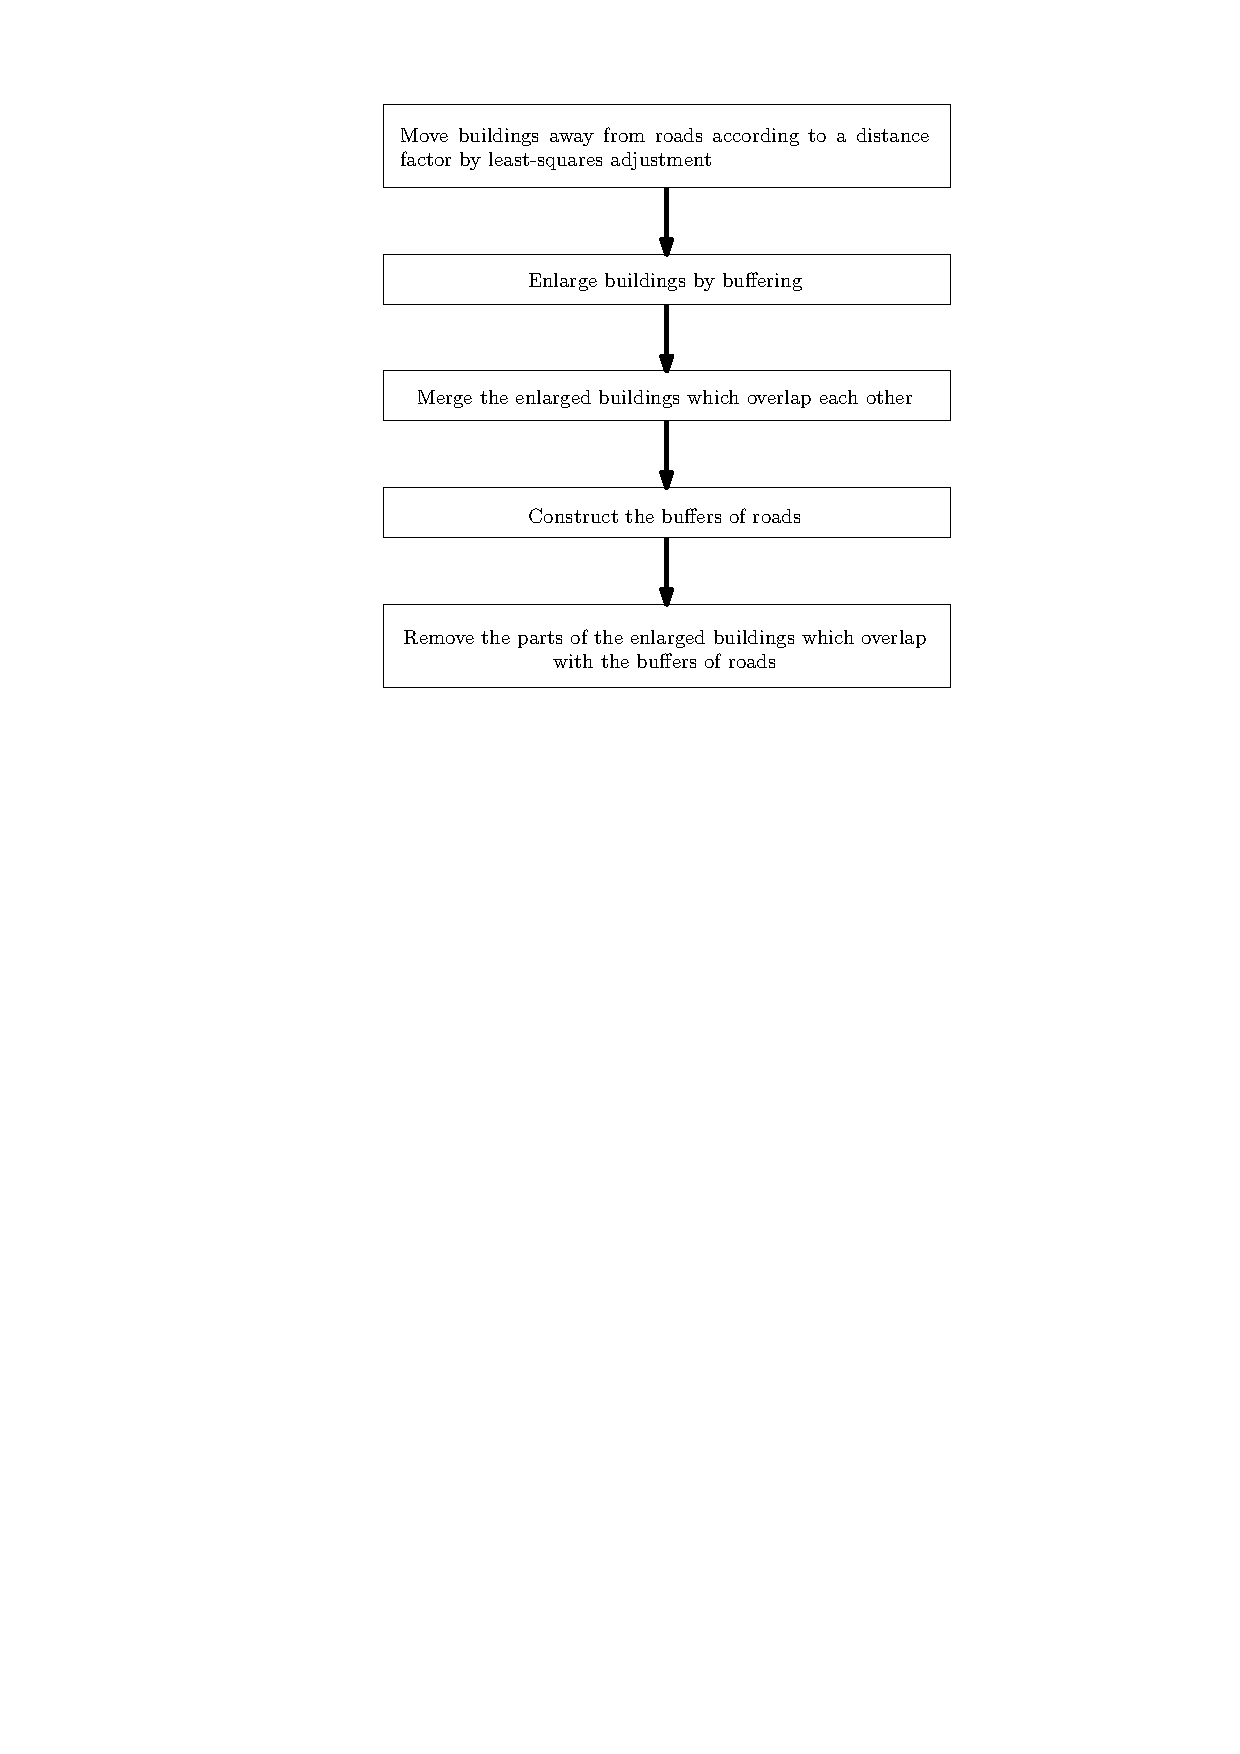
\includegraphics{Framework}
	\caption{Framework.}
	\label{fig:Framework}
\end{figure}



We discussed two ways of achieving continuous generalization of 
buildings. 

The first way is that we cover the smallest block at each step. 
Should we consider the density of the buildings? 
\marginalcomment{relevant comment. If small buildings exist in 
	all blocks, there will be small buildings remaining at small 
	scales in the blocks that have not been covered.}
A disadvantage 
is that some small buildings in a large block may exist very 
long.
Alternatively, we may cover two buildings together if they are 
close enough, say the distance is smaller than d. We can 
increase d so that we will cover more and more buildings 
together. To avoid overlap between two covers, we may need to 
use Voronoi diagrams of the original buildings. We can cover 
buildings without overlap if we always use a cover inside the 
Voronoi cells of these buildings. This idea about Voronoi cells 
is used in \textcite{vanGoethem2013}. We may need to try 
different 
possible covers. 
Unfortunately, this trying may be very time-consuming, probably 
NP-hard.

The second way is that we grow buildings by buffering with an 
increasing radius, and then merge the buffers overlapping each 
other. A disadvantage is that the corners of the buffers 
\marginalcomment{this may be avoided by using square buffers 
(the Minkowski sum is done with a square rather than a circle), 
don't know if it's available in ESRI products}
\marginalcomment{We can also think about the method described at 
%\url{http://stackoverflow.com/questions/1109536/an-algorithm-for-inflating-deflating-offsetting-buffering-polygons#}
 }
are not 
orthogonal anymore. Two kinds of buffer:


\begin{figure}[tb]
	\centering
	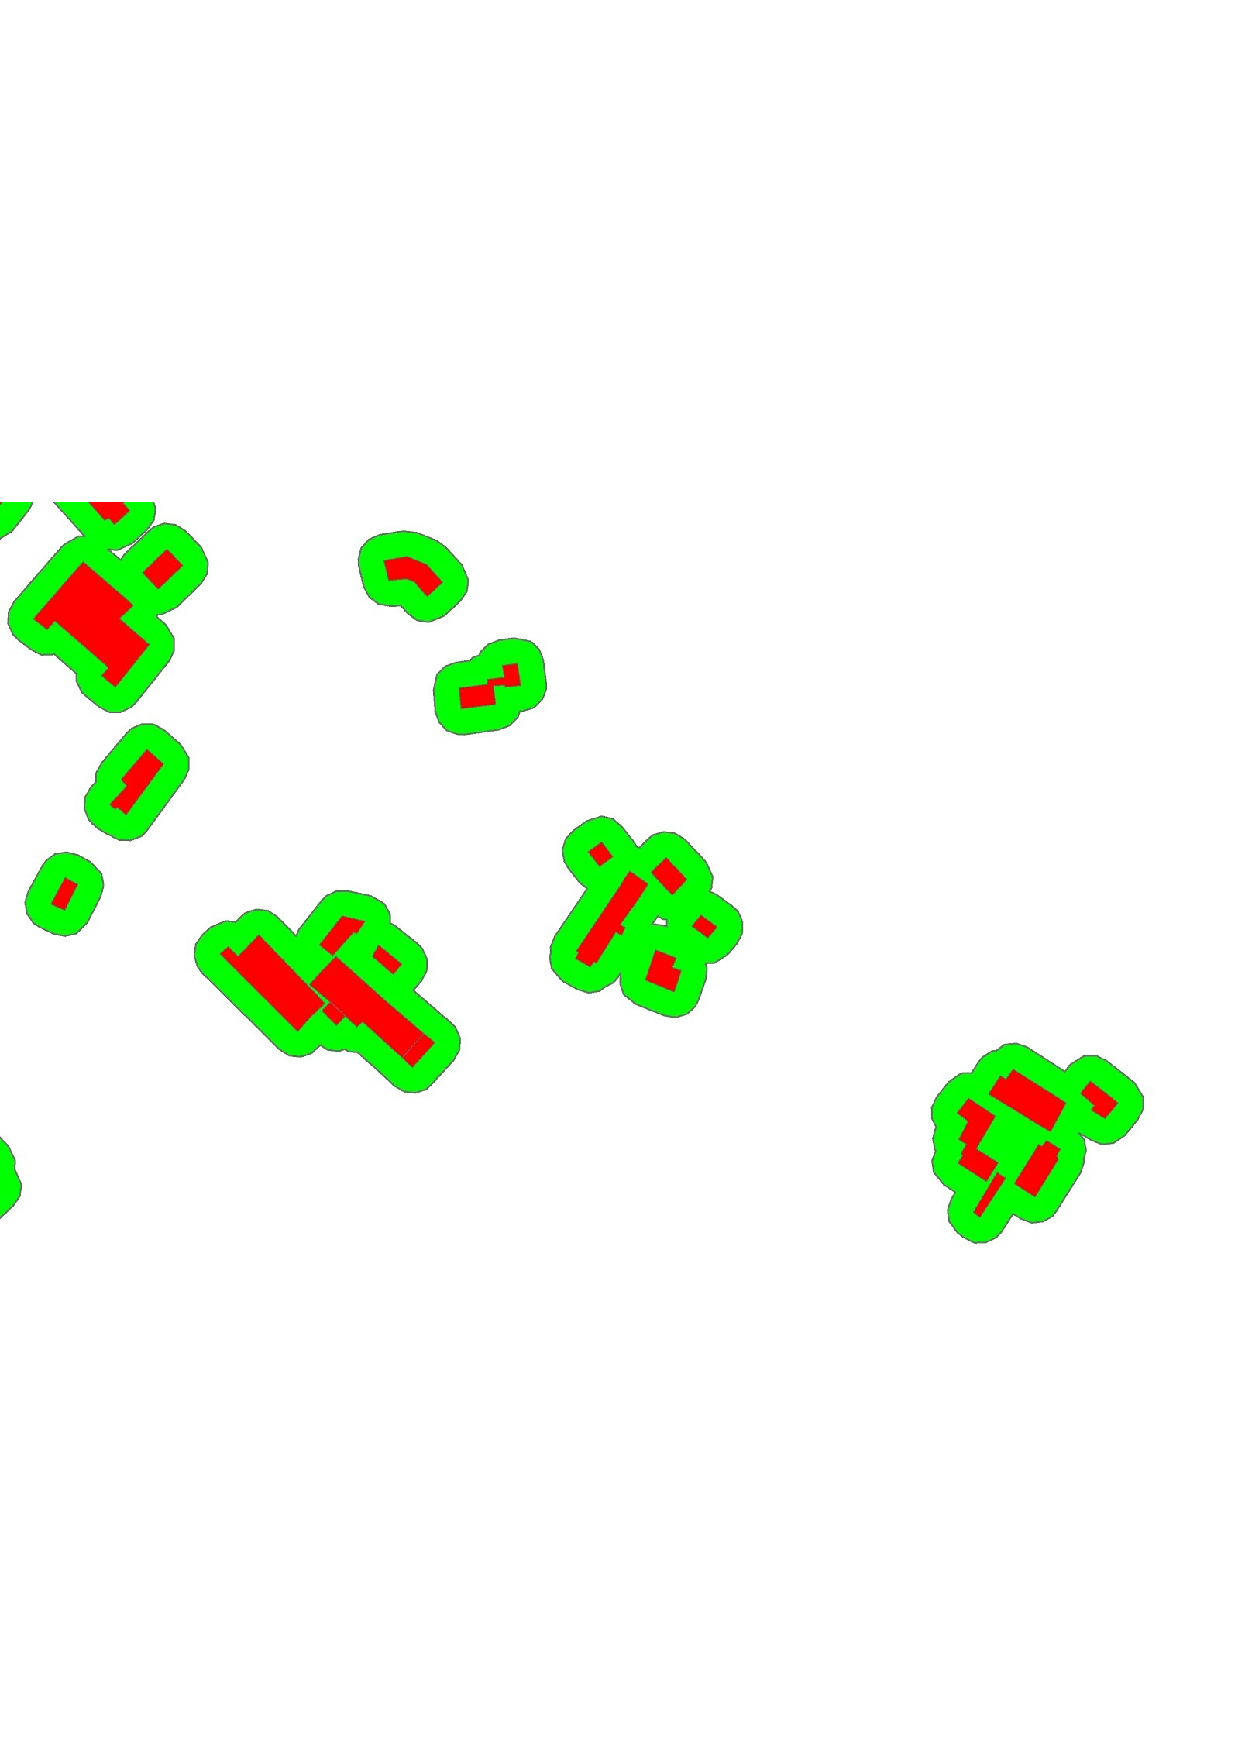
\includegraphics[width=\linewidth]{BufferRoundJoint}
	\caption{BufferRoundJoint.}
	\label{fig:BufferRoundJoint}
\end{figure}

\begin{figure}[tb]
	\centering
	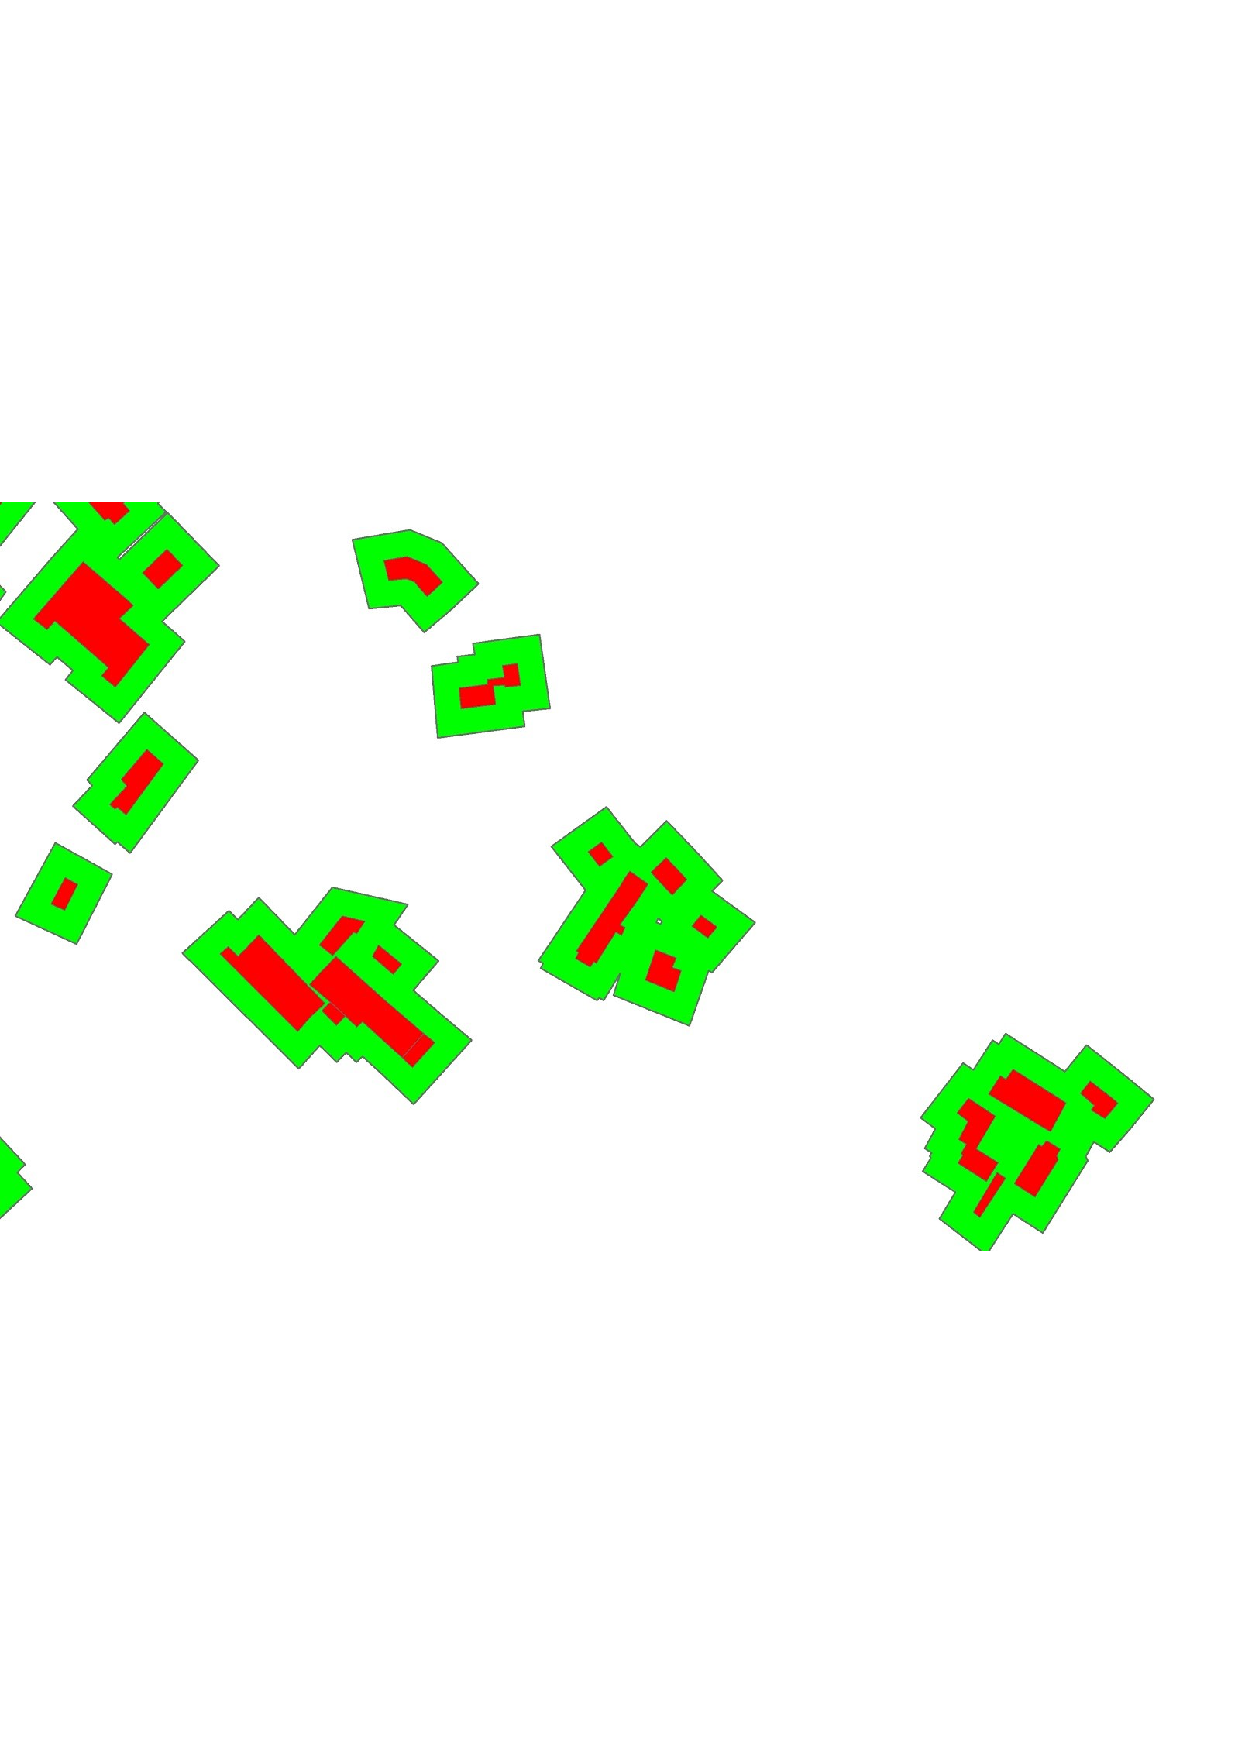
\includegraphics[width=\linewidth]{BufferMiterJoint}
	\caption{BufferMiterJoint.}
	\label{fig:BufferMiterJoint}
\end{figure}




A disadvantage of buffering based on miter joint is that the 
method is sensitive to noise. By sensitive, if there is a short 
edge at the end or a sharp corner, then the result will be very 
different to the case that there is no such short edge. In 
contrary, buffers based on round joint are continuous and stable.

This method should be easier to implement than the first method.
\marginalcomment{We can erode back in order to keep enough 
distance between buildings. The operator of growing and 
shrinking of buffers are mentioned in paper Automated Processing 
for Map Generalization with Modular Operator Services (Neun 
2009).
} 
We may not need to erode back after buffering. In this second 
strategy, undesired very small shapes or holes might appear at 
some point, and should be reverted until the growing totally 
collapses the hole or makes the small parts big enough. As 
buffers are not allowed to cross roads, we may clip some parts 
of the buffers off along the roads.
If we buffer with miter joint, it can happen that a very sharp 
angle yields a very long buffer. Fortunately, we do not have 
this situation so far. Otherwise, we may need to cut the long 
buffer at some point.
We may have small holes after buffering and merging the buffers 
of the buildings, which is not nice. See below as an example, 
where we can find a small “white” hole in the middle. We may 
simply fill out all the holes having small area.

\begin{figure}[tb]
	\centering
	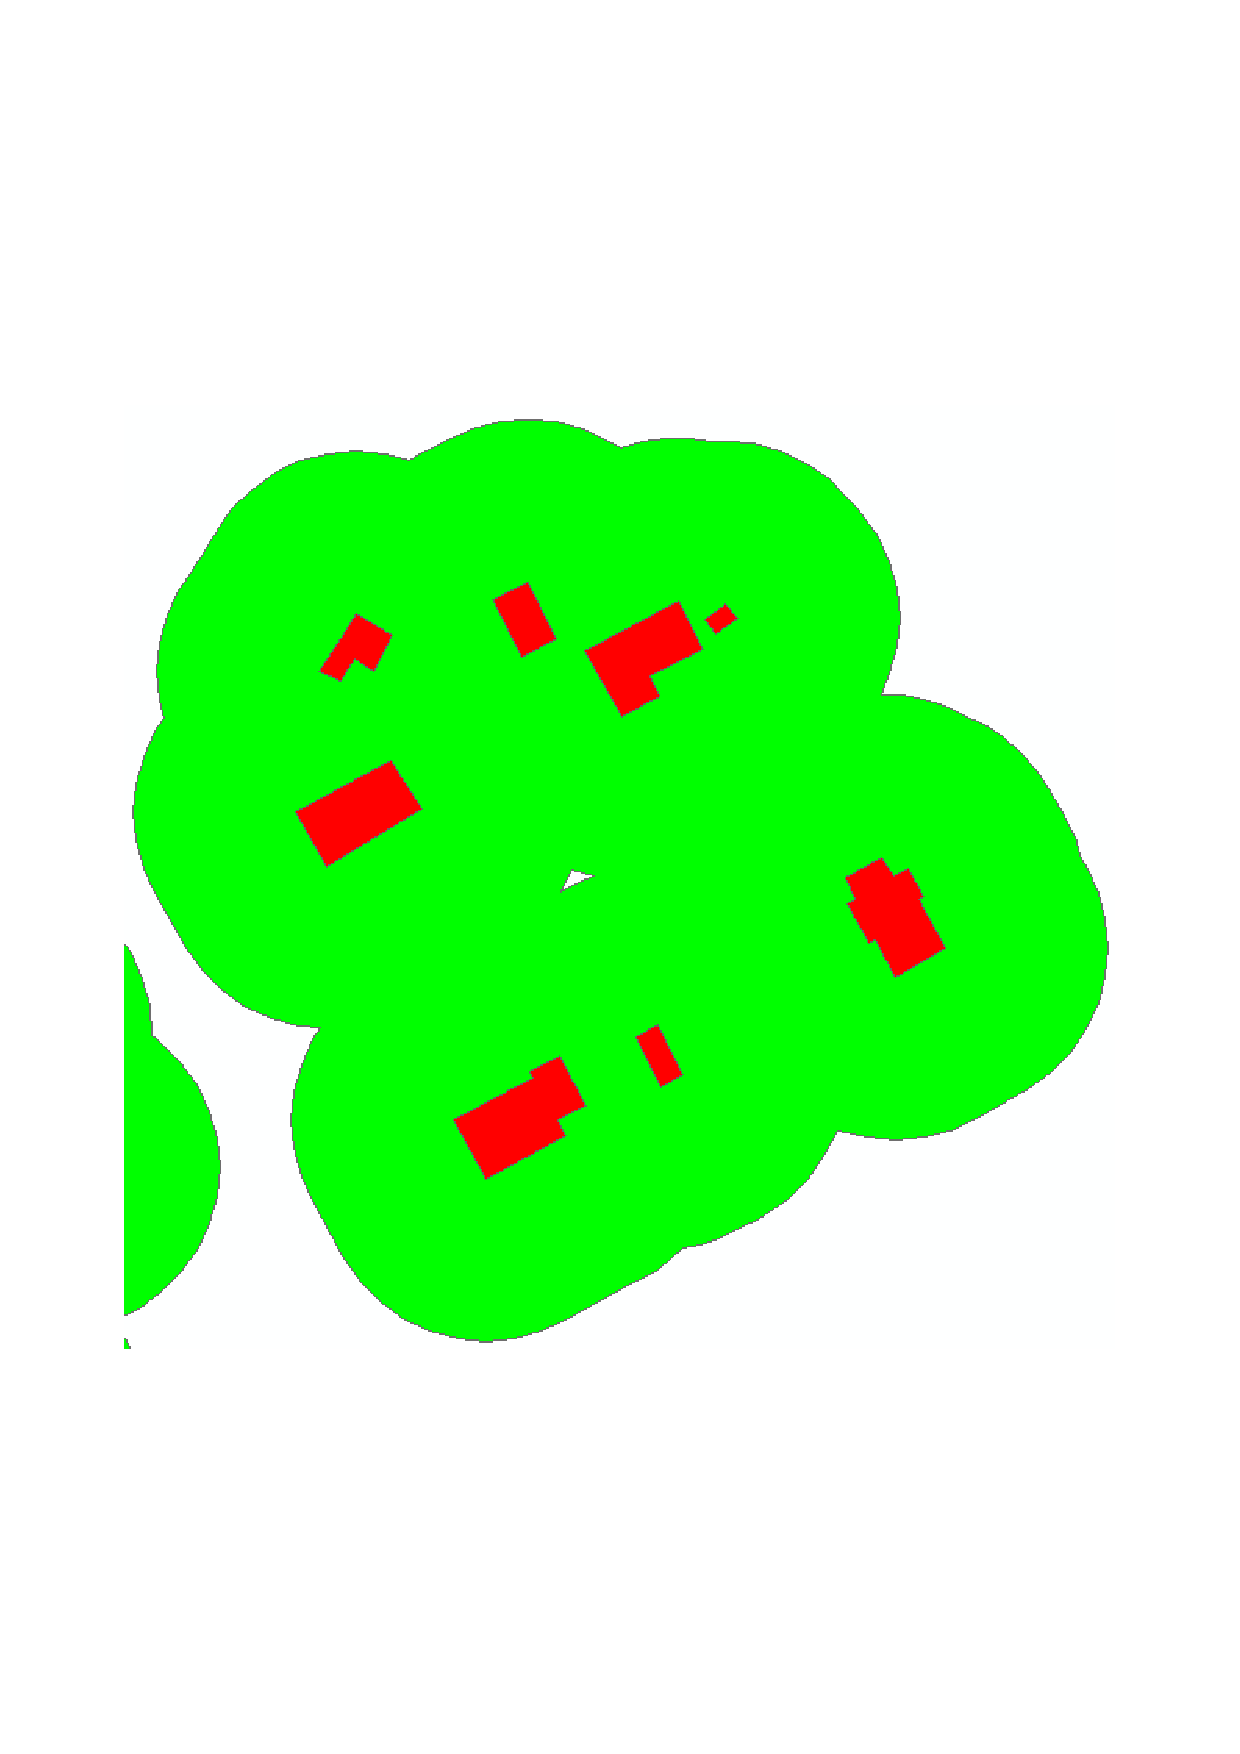
\includegraphics[width=\linewidth/2]{BufferWithHole}
	\caption{BufferWithHole.}
	\label{fig:BufferWithHole}
\end{figure}


We have two maps at different scales. We generalize the 
buildings on the larger-scale map, and we use the boundaries of 
the buildings on the smaller-scale map as the limits of the 
generalization (including growing).


We have a requirement that the buildings should not cross 
existing roads. Therefore, we need to cut the the enlarged 
buildings by the roads. If we do this cut, then some buildings 
may almost touch each other, but separated by roads. The 
too-close buildings will look ugly. To avoid the ugly 
performance, we should also make buffers for roads, and require 
that the enlarged buildings should be outside the buffers of the 
roads. Should we use the same radius that we used for enlarging 
buildings? With the buffers of roads growing, we may need to 
move enlarged buildings, otherwise, the enlarged buildings will 
overlap the buffers of roads. 
We may move by a method based on least-squares adjustment. In 
this method, we may assign large weight for keeping the distance 
between a road and a building. We may assign small weight for 
keeping the distance between buildings because buildings will be 
buffered and merged later.

We want to enlarge the buildings by a radius r, and require that 
the distance between any two buildings after the enlargement 
should be 2d at least. To achieve this aim, we first buffer the 
buildings by a radius r+d, and then buffer the enlarged 
buildings by a radius -d. Following is an example, where r=10 
and d=15.

Buffering the original buildings with radius 25

\begin{figure}[tb]
	\centering
	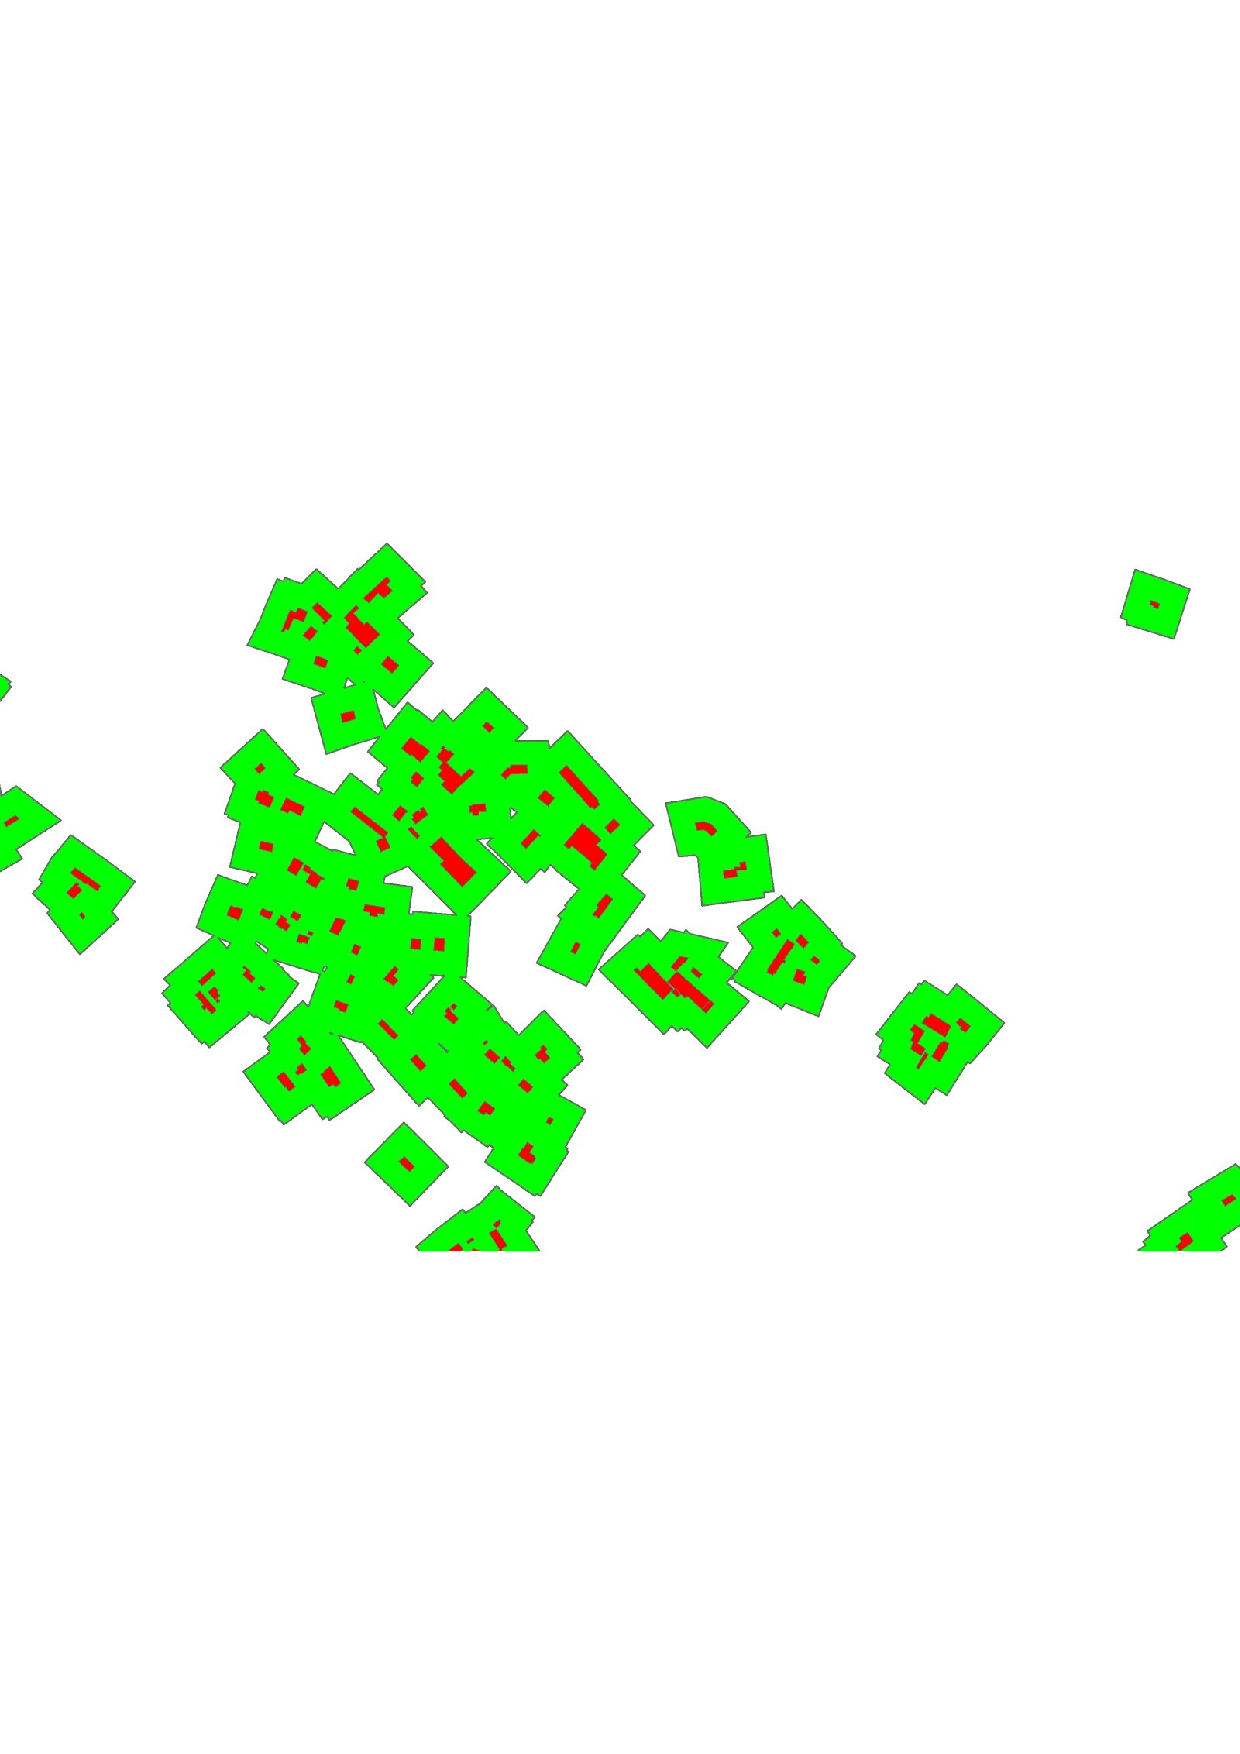
\includegraphics[width=\linewidth]{BufferRadius25}
	\caption{BufferRadius25.}
	\label{fig:BufferRadius25}
\end{figure}

Buffering the enlarged buildings with radius -15 (erosion). We 
call the result Map A. Unfortunately, we produced some spikes by 
this erosion. Since we used the miter joint and we allow the 
enlargements twice of radius r=10 away from the original 
buildings, the corners of the enlarged buildings can be 2r=20 
from the original buildings. After erosion, the smallest 
distance between two buildings can be as small as 0. I will give 
more details.

\begin{figure}[tb]
	\centering
	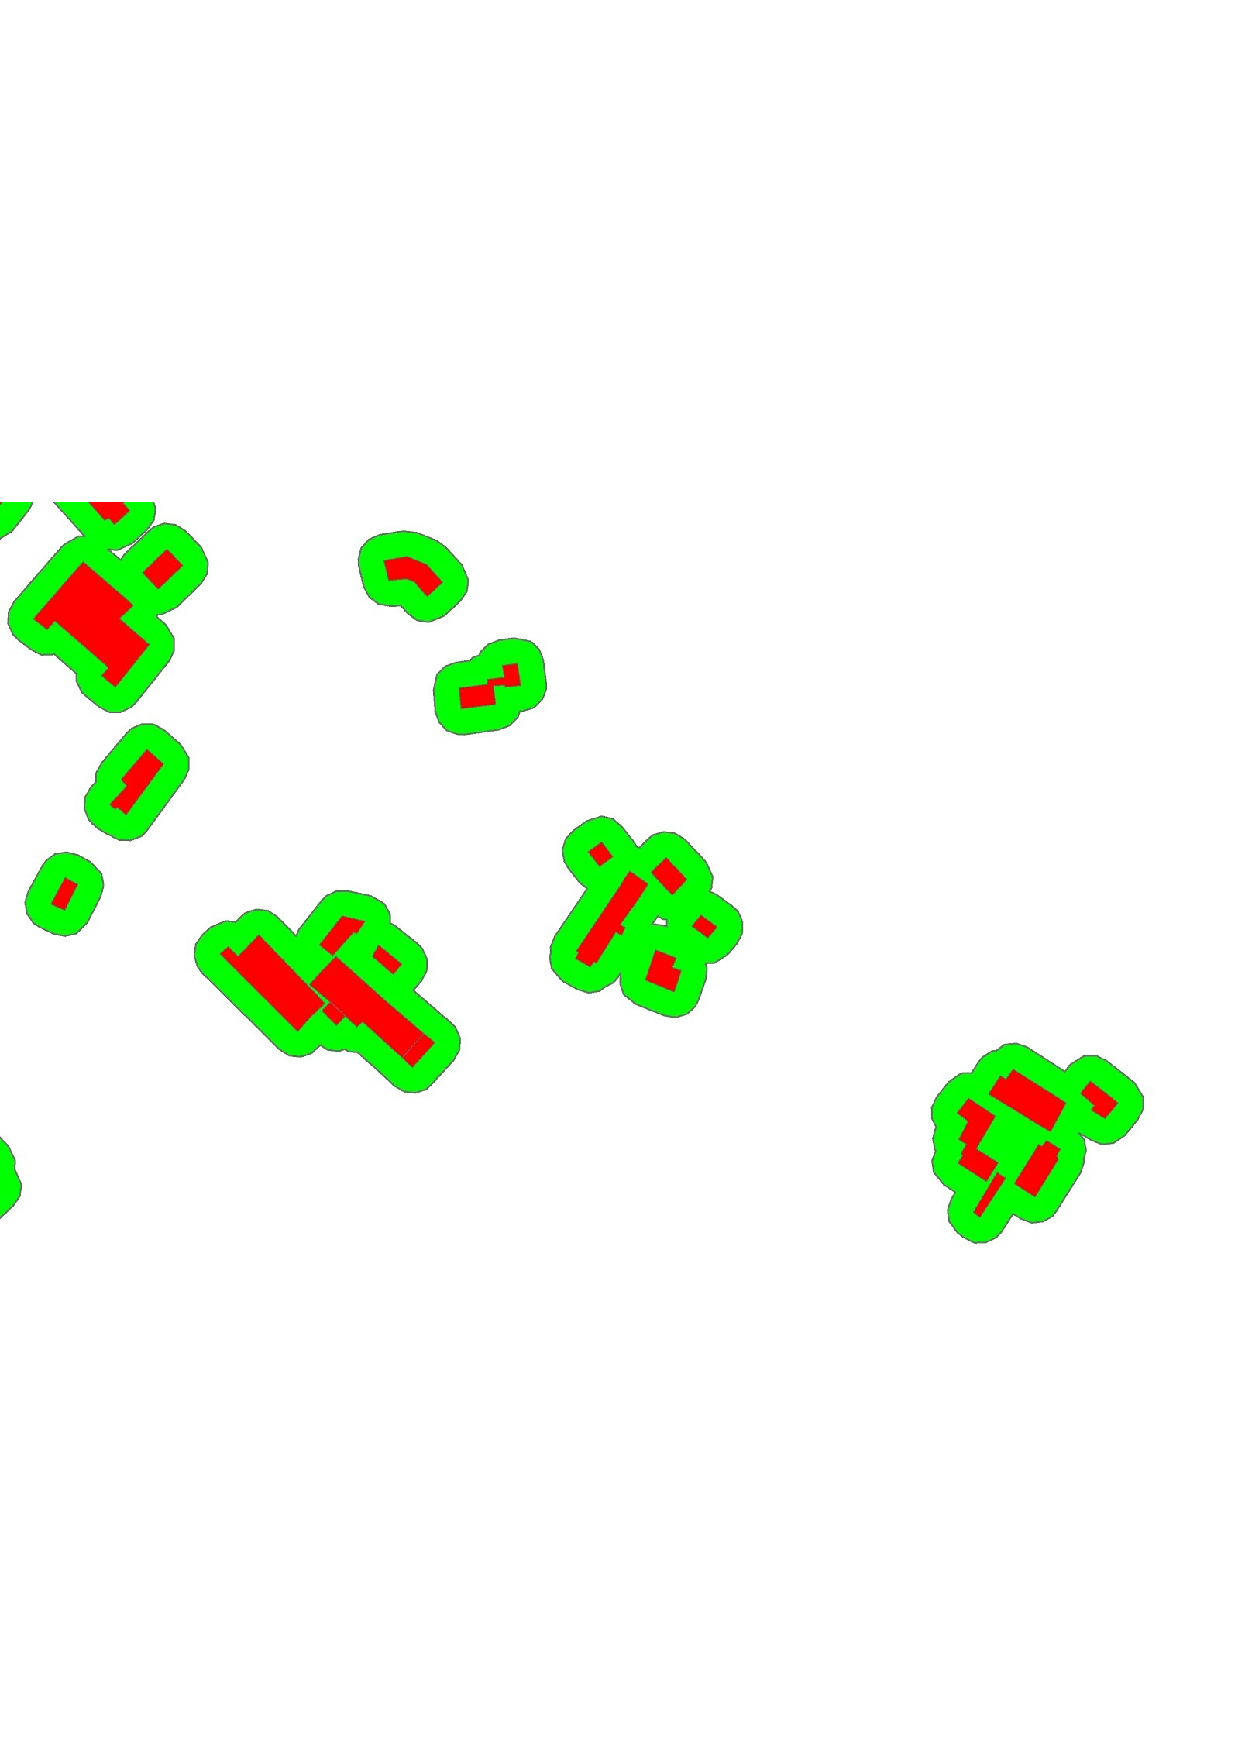
\includegraphics[width=\linewidth]{MapA}
	\caption{MapA.}
	\label{fig:MapA}
\end{figure}

Buffering the original buildings with radius 10. We call the 
result Map B.

\begin{figure}[tb]
	\centering
	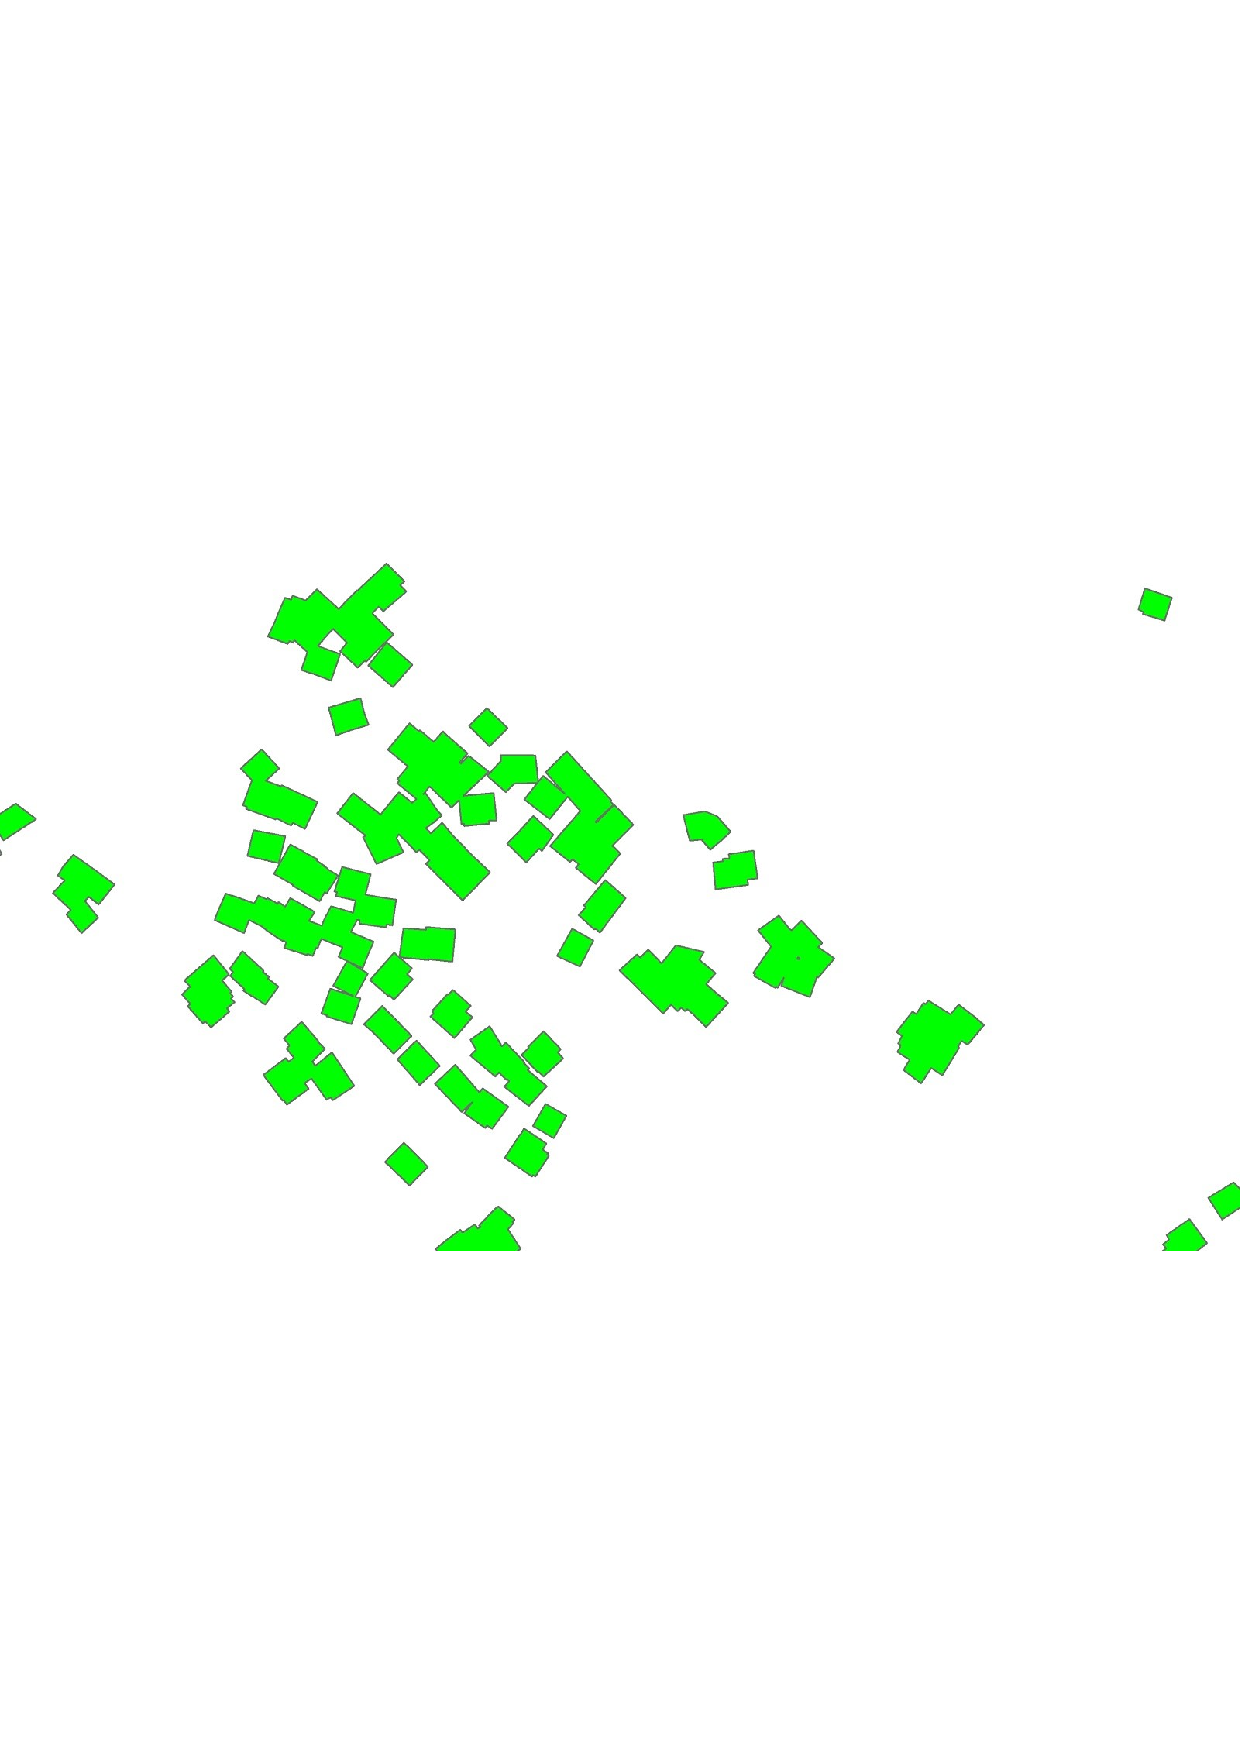
\includegraphics[width=\linewidth]{MapB}
	\caption{MapB.}
	\label{fig:MapB}
\end{figure}

To remove the spikes in Map A, we may subtract Map B from Map A. 
Then we get some leftovers in Map A. The outward triangles of 
the leftovers are the spikes which we want to remove. We 
subtract those outward triangles from Map A, which may guarantee 
that we will have removed the spikes in Map A.

To remove the spikes in Map A, Guillaume suggested that we could 
%buffer by a small value -ɛ, and then buffer again by ɛ.

Should we buffer from the original buildings or buffer from the 
buildings from the previous step?


Elimination
If every building should have area 4d2at least, we buffer 
buildings with radius xd (x<2). After the buffering, some too 
small buildings will be eliminated. The small buildings which 
manage to merge with other buildings may survive. The eliminated 
buildings should not participate in next buffering step, which 
uses larger d.




Issues regarding the data:

%How were the layers of data road_25k and road_100k produced?
%Was road_25k produced by surveying?
%Was road_100k generalized from road_25k?
%
%How were the layers of data building_15k, building_25k, 
%urban_area_50k, and urban_area_100k produced?
%Was building_15k produced by surveying?
%Was building_25k derived from building_15k by the methods 
%illustrated in paper Optimization Approaches for Generalization 
%and Data Abstraction (Sester, 2005)?
%Was urban_area_50k derived from building_15k by constructing 
%buffers and filling out the holes of the buffers?
%Was urban_area_100k derived from building_15k by constructing 
%buffers and filling out the holes of the buffers?

%\pagebreak[4]
%\newpage
\clearpage

\section{An idea of continuously generalising buildings}
We have an input map at scale $1:15 \mathrm{k}$.
We want to generate, by generalisation, $10$ maps which are at 
scale $1:20\mathrm{k}$, $1:25\mathrm{k}$, 
$1:30\mathrm{k}$, $\dots$, $1:65\mathrm{k}$.
We always produce a map by generalising the 
immediate-larger-scale map. For example, we produce the map at 
scale $1:25\mathrm{k}$ by generalising, instead of the input 
map, the map at scale $1:20\mathrm{k}$.
This production 
guarantees consistency. Namely, if a building does not exist on 
a map at a certain scale, then the building will never exist on 
a map at a smaller scale.

We have two requirements for an output map.
The first one is that the distance between two 
buildings should be at least $d_i=0.2 \mathrm{mm}/S_i$, where 
$S_i$ is the scale of map $i$.
The second requirement is that a building with area less than 
$A_i=0.16\mathrm{mm}^2/S^2_i$ should be eliminated. Roughly, a 
building with width less than 
$w_i=\sqrt{A_i}=0.4\mathrm{mm}/S_i$ should be eliminated.
In order to make sure that some small buildings will be 
eliminated, the radius $r_i$ that we use to buffer buildings 
should be smaller than $\frac{1}{2}w_i$. We simply use 
$r_i=\frac{1}{4}w_i$.
Our buildings may have been buffered with radius, in total, 
$r_{i-1}$ from previous steps.
Therefore, we only need to buffer with radius $r_i-r_{i-1}$ at 
the new 
step.

Our generalisation is as following $4$ steps:
\begin{enumerate}[label=(\alph*),leftmargin=2\parindent]
	\item We buffer buildings with 
	radius $\frac{1}{2}d_i+r_i-r_{i-1}$, and merge the buffers 
	overlapping each other.
	\item Then we buffer the results with $-\frac{1}{2}d_i$.
	\item In order to 
	remove some spikes from the buffering, we buffer the new 
	results with $-\epsilon_i$.
	\item To compensate, we buffer with $\epsilon_i$.	
\end{enumerate}
We simply set 
$\epsilon_i=\frac{1}{10}(r_i-r_{i-1})$. After these buffering 
operations, we eliminate the buildings with area less than 
$A_i$.







\section{Section Title}
\label{sec:AStarAlgorithm}

\mypar{Notation}
Text. 

\subsection{Text}
\label{sec:Formalizing}



\section{Conclusions}
\label{sec:Conclusions}

Because of our aggregation with skeletons and original 
buildings, we may have too many details in the intermediate 
results.

Some buildings are too small to be eroded. We have to generate 
squares or MBR?

To make it more efficient for on line displaying, we may need 
some external memories. First, we store the data at some key 
scales so that we may start a generalization from the immediate 
larger scale; $O(n)$ space. Second, we store the target shape 
for each building; $O(n)$ space. Third, we store the aggregation 
time and the target form for the aggregated shape; $O(n^2)$ 
space if we count vertex number.
%
The displaying time is dependent on buffering and clipping. The 
two operators are from library Clipper. The efficiency of the 
buffering function of this library has been evaluated by 
\textcite{Palfrader2015}.

One can also discuss about our growing speed.

\printbibliography
%\bibliographystyle{plainnat}
%%	\bibliography{References}
%\input{referenc}
\end{document}